\documentclass[darkblue]{beamer}
\usepackage[utf8]{inputenc} % codificacao de caracteres
\usepackage[T1]{fontenc}    % codificacao de fontes
\usepackage[brazil]{babel}  % idioma
\usepackage{csvsimple}
\usepackage{minted}
\usetheme{Ilmenau}         % tema
\setbeamertemplate{mini frames}{}
\setbeamertemplate{headline}{}
\setbeamertemplate{footline}[frame number] % numero de slides
\beamertemplatenavigationsymbolsempty % Desativando os botoes de navegacao
\hypersetup{pdfpagemode=FullScreen} % Tela cheia

% Titulo
\title{Implementação Naïve Bayes: Python}
\author{Mateus Tarcinalli Machado}
\institute{Introdução ao Aprendizado de Máquina \\ Prof. Dr. José Augusto Baranauskas} % opcional
\date{\today}

\begin{document}

    \begin{frame}
    	\titlepage
    \end{frame}
    
    \begin{frame}{Apresentação}
    	\tableofcontents
    \end{frame}
    
    \section{Apresentação}
    
    \begin{frame}{Introdução}
        \begin{block}{Trabalho para a disciplina Introdução ao Aprendizado de Máquina:}
            Implementação Naïve Bayes: Python
        \end{block}
        \begin{block}{Motivação:}
            ALMANSA, Luciana Farina et al. Information learned from monitoring microblogs during the 2014 seasonal flu vaccination in Brazil. In: 2014 IEEE 10th International Conference on e-Science. IEEE, 2014. p. 65-66.
        \end{block}
    \end{frame}
    
    \section{Módulos Utilizados}
    
    \begin{frame}{Módulos Utilizados}
    	\inputminted{python}{cod01.py}
    \end{frame}
    
    \section{Classe}
    
    \begin{frame}{Classe}
    	\inputminted{python}{cod02.py}
    \end{frame}
    
    \subsection*{Carregar Dados}
    
    \begin{frame}{Carregar}
    	\inputminted{python}{cod03.py}
    \end{frame}
    
    \subsection*{Treinar}
    
    \begin{frame}[allowframebreaks]{Treinar}
    	\inputminted{python}{cod05.py}
    \end{frame}
    
    \subsection*{Predizer}
    
    \begin{frame}[allowframebreaks]{G}
    	\inputminted{python}{cod06.py}
    \end{frame}
    
    \begin{frame}[allowframebreaks]{Predizer}
    	\inputminted{python}{cod07.py}
    \end{frame}
    
    \subsection*{Gráfico Fronteira}
    
    \begin{frame}[allowframebreaks]{Gráfico}
    	\inputminted{python}{cod08.py}
    \end{frame}
    
    \section{Validação Cruzada}
    
    \begin{frame}[allowframebreaks]{Validação Cruzada}
    	\inputminted{python}{cod09.py}
    \end{frame}
    
    \section{Dataset Tenis}
    
    \begin{frame}[allowframebreaks]{Dataset Tenis}
        \csvautotabular{tenis.csv}
    \end{frame}
    
    \begin{frame}[allowframebreaks]{Validação Cruzada}
    	\inputminted{python}{cod10.py}
    \end{frame}
    
    \begin{frame}[allowframebreaks]{tenis2.modelo}
    	\inputminted{python}{cod11.py}
    \end{frame}
    
    \section{Gráficos de Fronteira}
    
    \begin{frame}{iris: 2 dimensões}
        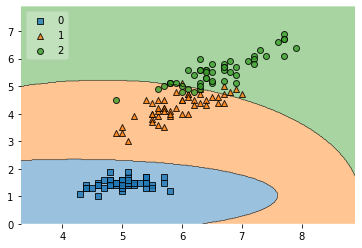
\includegraphics[width=\textwidth]{output_35_0.png}
        \centerline{Acurácia  : 88.89 \%}
    \end{frame}
    
    \begin{frame}{cassini}
        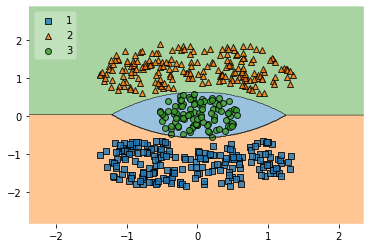
\includegraphics[width=\textwidth]{output_39_0.png}
        \centerline{Acurácia  : 100.00 \%}
    \end{frame}
    
    \begin{frame}{circle}
        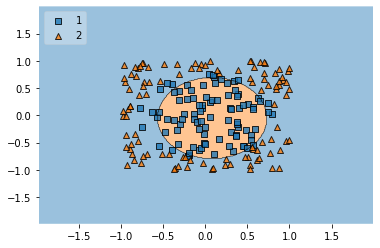
\includegraphics[width=\textwidth]{output_43_0.png}
        \centerline{Acurácia  : 95.00 \%}
    \end{frame}
    
    \begin{frame}{hypercube}
        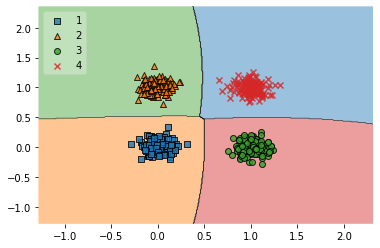
\includegraphics[width=\textwidth]{output_47_0.png}
        \centerline{Acurácia  : 100.00 \%}
    \end{frame}
    
    \begin{frame}{ringnorm}
        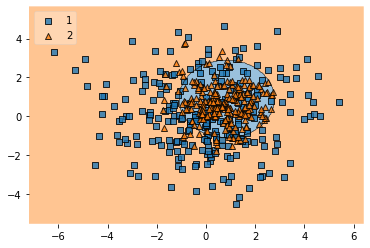
\includegraphics[width=\textwidth]{output_51_0.png}
        \centerline{Acurácia  : 80.67 \%}
    \end{frame}
    
    \begin{frame}{shapes}
        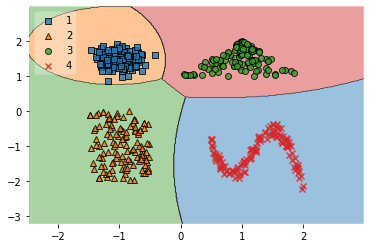
\includegraphics[width=\textwidth]{output_55_0.png}
        \centerline{Acurácia  : 100.00 \%}
    \end{frame}
    
    \begin{frame}{simplex}
        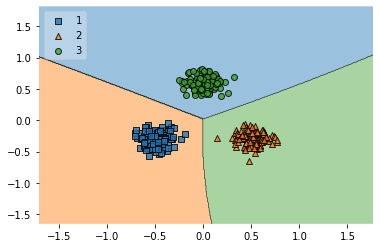
\includegraphics[width=\textwidth]{output_59_0.png}
        \centerline{Acurácia  : 100.00 \%}
    \end{frame}
    
    \begin{frame}{smiley}
        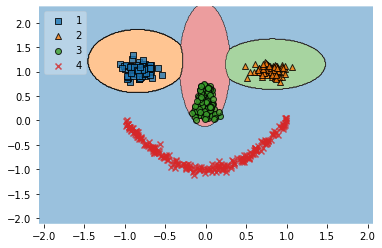
\includegraphics[width=\textwidth]{output_63_0.png}
        \centerline{Acurácia  : 100.00 \%}
    \end{frame}
    
    \begin{frame}{spirals}
        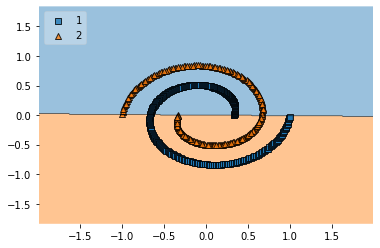
\includegraphics[width=\textwidth]{output_67_0.png}
        \centerline{Acurácia  : 46.00 \%}
    \end{frame}
    
    \begin{frame}{spirals}
        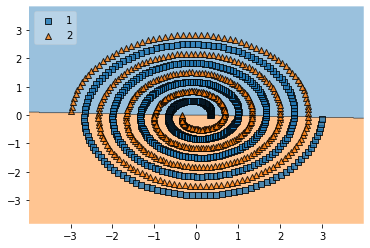
\includegraphics[width=\textwidth]{output_71_0.png}
        \centerline{Acurácia  : 46.67 \%}
    \end{frame}
    
    \begin{frame}{threenorm}
        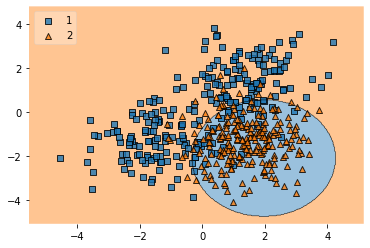
\includegraphics[width=\textwidth]{output_75_0.png}
        \centerline{Acurácia  : 90.00 \%}
    \end{frame}
    
    \begin{frame}{twonorm}
        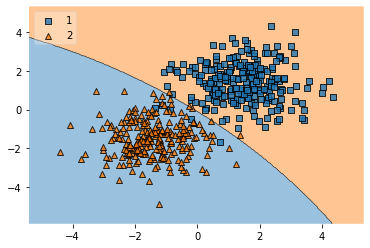
\includegraphics[width=\textwidth]{output_79_0.png}
        \centerline{Acurácia  : 98.67 \%}
    \end{frame}
    
    \begin{frame}{xor d=2}
        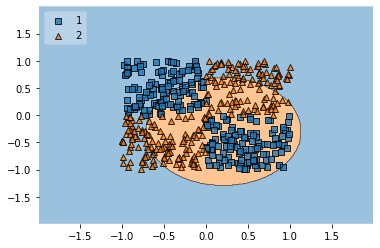
\includegraphics[width=\textwidth]{output_83_0.png}
        \centerline{Acurácia  : 52.00 \%}
    \end{frame}
    
    \section{Carregar Texto}
    
    \begin{frame}[allowframebreaks]{Carregar Texto}
    	\inputminted{python}{cod04.py}
    \end{frame}
    
    \section{Análise de Sentimentos}

    \begin{frame}{Dataset Amazon}
        \csvautotabular{amazon.csv}
        \begin{block}{}
        print(len(amazon.dados))
        
        \# 1000
        
        print(len(amazon.dados[0]))
        
        \# 1629
        
        print(amazon.dados[0][:10])
        
        \# ['pn0', 'pn1', 'pn2', 'pn3', 'pn4', 'pn5', 'pn6', 'pn7', 'pn8', 'pn9']
        \end{block}
        \begin{block}{}
        Conj Teste: 300
        
        Acertos   : 233
    
        Acurácia  : 77.66666666666666 \%
        \end{block}
    \end{frame}
    
    \begin{frame}{Dataset IMDB}
        \csvautotabular{imdb.csv}
        \begin{block}{}
        Conj Teste: 300
        
        Acertos   : 224
    
        Acurácia  : 74.66666666666667 \%
        \end{block}
    \end{frame}
    
    \begin{frame}{Dataset Yelp}
        \csvautotabular{yelp.csv}
        \begin{block}{}
        Conj Teste: 300
        
        Acertos   : 229
    
        Acurácia  : 76.33333333333333 \%
        \end{block}
    \end{frame}
    
    \begin{frame}
    	\label{perg}
    	\begin{center} 
    		\Huge Perguntas?
    	\end{center} 
    \end{frame}
    
    \begin{frame}
    	\begin{center} 
    		\Huge Muito Obrigado!
    	\end{center} 
    \end{frame}

\end{document}